\documentclass[conference]{IEEEtran}
\IEEEoverridecommandlockouts
% The preceding line is only needed to identify funding in the first footnote. If that is unneeded, please comment it out.
%Template version as of 6/27/2024

\usepackage{cite}
\usepackage{amsmath,amssymb,amsfonts}
\usepackage{algorithmic}
\usepackage{graphicx}
\usepackage{textcomp}
\usepackage{xcolor}
\usepackage{tabularx}
\usepackage{booktabs}
\usepackage{tabularx}
\usepackage{geometry}
\usepackage{hyperref}
\def\BibTeX{{\rm B\kern-.05em{\sc i\kern-.025em b}\kern-.08em
    T\kern-.1667em\lower.7ex\hbox{E}\kern-.125emX}}
\begin{document}

\title{COS 711 Assignment 2 Report\\
}

\author{\IEEEauthorblockN{Nathan Opperman}
\IEEEauthorblockA{ \\
u21553832@tuks.co.za}
\IEEEauthorblockA{ \\
github\: \url{https://github.com/nathanMils/711_Ass1}}
}

\maketitle

\begin{abstract}
This assignment explores the classification of almond types utilizing a Kaggle dataset comprising 2,803 samples, each defined by fourteen morphological attributes. The study examines various optimization techniques and hybrid methods to enhance classification performance. By implementing k-fold cross-validation and hyperparameter tuning, the effectiveness of different optimizers is assessed, revealing significant insights into their impact on model accuracy.
\end{abstract}

\section{Introduction}
In this assignment, I will be evaluating and comparing various hyperparameters and with a focus specifically training algorithms . The goal is to understand the trade-offs of each approach by exploring different configurations of learning rates, batch sizes, and network architectures. I aim to identify the optimal conditions that yield the best performance.\\

Firstly before any training can be done, data must be prepared and so I will first go over how the data has been analysed and transformed in order to ensure that data is correctly scaled, formatted and selected as to not hinder model performance.\\

Next I will conduct hyperparameter tuning can have a great affect, as the right choices can drastically enhance model performance while the wrong ones can lead to overfitting or underfitting amongst other issues. I will leverage techniques such as K-fold cross-validation and grid search to assess and compare the impact of these hyperparameters on model performance. At the same time, I will investigate various gradient based training algorithms, including gradient descent variants and advanced optimization techniques like Adam and Rprop. Each algorithm will be analysed in terms of its convergence speed and solution quality, allowing for a deep understanding of their applicability to different datasets and tasks.\\

The results of these experiments will then be presented as to highlight certain significant metrics such as accuracy and loss. By comparing these metrics across different configurations, I aim to provide insight into the design of a robust neural network. Ultimately, this report will not only demonstrate the importance of careful hyperparameter selection and algorithm choice but also demonstrate my own understanding of neural networks in general.


\section{Background}
In this section, I will attempt to provide a high-level discussion of the problem domain of multi-class classification, as well as the algorithms and approaches I used thoughout the course of this project.\\
\subsection{Multi-class Classification}
Multi-class classification is a learning task where the objective is to categorize instances into more than two classes, in our case three classes (SANORA, MAMRA, REGULAR). There are many different techniques and approaches for multi-class classification such as neural networks, decision trees (DT) \cite{breiman2017classification}, k-Nearest Neighbor \cite{bay1998combining},and Support Vector Machines (SVM) \cite{brereton2010support}. Multi-class classification and these approaches are discussed in more detail in \cite{aly2005survey}. In this project, I will utilize the neural network approach which applies the softmax activation function in the output layer to generate class probabilities for each of the three almond types.

\subsection{K-Fold Cross Validation and Grid Search}
Hyperparameter optimization is an important step in machine learning, involving tuning parameters that influence the performance of models. K-Fold Cross Validation is a robust technique used to evaluate model performance by partitioning the dataset into $k$ sets and training the model on $k-1$ sets while validating/training on the remaining set. 

Grid search is a systematic approach for hyperparameter optimization, where a set of parameters is created, and the model is trained and evaluated on all possible combinations of these parameters. Together, these methods ensure that the best-performing parameter configuration is identified.

\subsection{Training Algorithms - SGD}
Stochastic Gradient Descent (SGD), or stochastic approximation, is a common optimization/training algorithm for neural networks \cite{zhou2021convergence} in both regression and classification. Unlike standard gradient descent, which computes the gradients based on the dataset in its entirety, SGD updates the model parameters using only a single example/batch for each iteration. This improves the speed of the training process. However, one issue is that the updates can be noisy which can potentially lead to fluctuations in the learning process. However, stochastic gradient decent is still popular due to its ability to escape local minima.

\subsection{Training Algorithms - Adam}
Adam (Adaptive Moment Estimation) is a modern, advanced optimization/training algorithm that combines the benefits of two other extensions of stochastic gradient descent, RMSProp and momentum. It computes adaptive learning rates for each parameter by keeping an exponentially decaying average of past gradients (first moment) and squared gradients (second moment). This adaptive behaviour aids in converging to a solution. The benefits of Adam include fast convergence and robustness.

\subsection{Training Algorithms - Rprop}
Resilient Backpropagation (Rprop) is an optimization/training algorithm that improves upon the standard backpropagation algorithm  by instead focusing on the sign of the gradient rather than its magnitude. This helps Rprop overcome issues like vanishing gradients and leads to faster convergence, making it effective for  more complex error landscapes.

There are many other advanced/simple optimization/training algorithms in the field of machine learning \cite{math11112466}. However in this assignment I will  be focusing solely on these three: SGD, Adam and Rprop.

\subsection{Hybrid Learning}
Hybrid learning combines multiple learning approaches or algorithms to leverage their individual strengths. In the context of this project, hybrid learning may involve using ensemble methods, where multiple models are trained independently and their predictions are combined, or integrating different optimization techniques to enhance training performance. This approach can lead to improved model accuracy and robustness, particularly in complex classification tasks like almond classification.

summerise the remainder of the paper

\section{Experimental Set-Up}
In this section, I will outline the approaches and strategies utilized throughout this assignment and provide rationale for the various choices made regarding data preparation hyperparameters and hybrid learning. \\

Firstly I start with data preparation, then justify my choices for hyperparameters I plan to use for all optimization algorithms, namely: weight initialization, activation functions, loss function and NN architecture. I will then explain the three optimization/training algorithms I intend to compare, along with my implementation for hybrid learning. Finally I will go over the hyperparameters I intend to tune and how I will do so. \\ 
\subsection{Data Preparation}
Data preparation is the first step of any learning process and is vital to enhancing the performance of any neural network models.

\subsection{Dataset Description}
The "Almond Types Classification" dataset was collected from Kaggle and comprises a total of 2,803 almonds. Each almond is described by fourteen attributes, including its ID and Type. The dataset features 2D images of almonds captured in three different orientations: upright, on its side, and laid on its back. The primary objective of this dataset is to classify each almond into one of three categories: SANORA, MAMRA, and REGULAR. In total the dataset includes the following attributes: Id, Length, Width, Thickness, Area, Perimeter, Roundness, Solidity, Compactness, Aspect Ratio, Eccentricity, Extent, Convex hull, and Type (SANORA, MAMRA, REGULAR).\\
\textbf{Class Distribution}\\
The almond types are distributed as follows:
\begin{itemize}
	\item \textbf{SANORA}: 943 samples (33.64\%)
	\item \textbf{MAMRA}: 933 samples (33.39\%)
	\item \textbf{REGULAR}: 927 samples (33.07\%)
\end{itemize}
This class distribution is rather fair so there should not be any issue regarding class bias at this point.
\begin{table*}[h]
    \centering
    \caption{Statistical Summary of Features with Missing Values}
    \label{tab:dataset_stats}
    \begin{tabularx}{\textwidth}{@{}lXXXXXXXXX@{}}
        \toprule
        Feature & Count & Mean & Std Dev & Min & 25\% & 50\% & 75\% & Max & Missing Values \\ 
        \midrule
        Length (major axis)        & 2803   & 1401.00   & 809.30   & 0.00      & 700.50     & 1401.00   & 2101.50   & 2802.00 & 857 \\
        Width (minor axis)        & 1946   & 290.61    & 62.72    & 151.34    & 245.97    & 279.88    & 330.51    & 515.35 & 942 \\
        Thickness (depth)         & 1799   & 109.71    & 18.94    & 59.49     & 97.09     & 110.28    & 121.39    & 181.85 & 1004 \\
        Area                       & 2803   & 26511.12  & 13782.56 & 6037.00   & 16211.50  & 23440.50  & 33451.00  & 89282.50 & 0 \\
        Perimeter                  & 2803   & 743.86    & 230.63   & 311.56    & 571.73    & 707.49    & 878.90    & 1864.95 & 0 \\
        Roundness                  & 1946   & 0.47      & 0.12     & 0.17      & 0.38      & 0.47      & 0.58      & 0.70 & 857 \\
        Solidity                   & 2803   & 0.96      & 0.04     & 0.72      & 0.94      & 0.97      & 0.98      & 0.99 & 0 \\
        Compactness                & 2803   & 1.83      & 0.79     & 1.16      & 1.36      & 1.58      & 1.97      & 9.66 & 0 \\
        Aspect Ratio               & 1004   & 1.75      & 0.21     & 1.40      & 1.61      & 1.71      & 1.83      & 2.73 & 1799 \\
        Eccentricity               & 1004   & 0.81      & 0.04     & 0.70      & 0.78      & 0.81      & 0.84      & 0.93 & 1799 \\
        Extent                     & 2803   & 0.72      & 0.05     & 0.45      & 0.70      & 0.73      & 0.76      & 0.85 & 0 \\
        Convex hull (convex area) & 2803   & 27696.22  & 14237.35 & 6355.00   & 17088.50  & 24589.00  & 34863.25  & 90642.50 & 0 \\ 
        \bottomrule
    \end{tabularx}
\end{table*}
\subsection{Data Cleaning - Missing Values}
As you can see in Table \ref{tab:dataset_stats}, one of the main issues of this dataset are the attributes: Length, Width and Thickness, whereby each almond is missing exactly one of these attributes. Specifically 30.57\% are missing Length, 33.61\% are missing Width and 35.82\% are missing Thickness. This is clearly an extensive amount of missing information, and requires care consideration to ensure that information loss is kept to a minimal while without degrading the data.
\newline \\
To address this I decided to utilize the iterative imputer (IterativeImputer) from the scikit-learn library. This is a multivariate imputer that estimates each feature based on all the others. It uses a strategy for imputing values by modeling each feature with missing values as a function of others in a round-robin like fashion.
\newline \\
It is important to clarify that features like Roundness, Aspect Ratio, and Eccentricity, which depend on Length, Width, and Thickness, will be excluded from the imputation process. Including these dependent features would not provide valid imputations, as their values rely on the very attributes that are missing. Instead, I will compute these dependent attributes after imputation, ensuring accurate calculations based on the newly estimated values.
\newline \\
Furthermore, to enhance the reliability of computing Roundness, which is derived from both Length and Area. The issue here is that Area is dependent on the angle of the image, I introduced a temporary feature, Area\_Length. The reason being is that Area is obviously dependent on the angle of the image taken, meaning it is highly dependent on weather length is present. So computing Roundness using Area that is not consistent with length will cause Roundness to be inconsistent. However Area\_Length will retain the value of Area when Length is available, while remaining NaN when Length is absent. The IterativeImputer will then impute missing values for Area\_Length, providing a more stable basis for accurately calculating Roundness.

\subsection{Bias Handling}
Neural networks are data-driven models, meaning their performance and predictions are highly dependent on the data they are trained on. This means that if our training data contains bias, the model will likely learn this bias and propagate it in its predictions on unknown data. This is a particularly important issue, luckily this dataset appears to represent each class equally with 943 (33.64\%) SANORA almonds, 933 (33.39\%) MAMRA almonds and 927 (33.07\%) REGULAR almonds. Therefore each class is represented almost equally and so class bias should not be an issue.

\subsection{Data Transformation - Encoding}
In the dataset, the only non-numerical feature is the class attribute 'Type', which denotes the type of almond. Since neural networks require numerical input, it is essential to transform this categorical variable into a numerical format. For this purpose, I utilized label encoding, assigning a unique integer to each category. However, the integer values are treated as indices, effectively simulating one-hot encoding. 

Label encoding involves converting each unique category in a nominal variable into a corresponding integer value. While this method is typically employed for ordinal data, in this case, the integer values are used as indices for the model. This allows the objective function to correctly interpret these values while maintaining the nominal nature of the data. For the 'Type' feature, which includes three unique categories: SANORA, MAMRA, and REGULAR, the encoding is illustrated in Table \ref{tab:encoding_matrix}.

\begin{table}[h]
    \centering
    \caption{Encoding}
    \small
    \begin{tabular}{|p{1.5cm}|p{0.5cm}|p{0.5cm}|p{0.5cm}|p{1.1cm}|}
        \hline
        \textbf{Type} & \textbf{1} & \textbf{2} & \textbf{3} & \textbf{encoding} \\
        \hline
        SANORA    & 1 & 0 & 0 & 1\\
        \hline
        MAMRA     & 0 & 1 & 0 & 2\\
        \hline
        REGULAR 	 & 0 & 0 & 1 & 3\\
        \hline
    \end{tabular}
    \label{tab:encoding_matrix}
\end{table}

\subsection{Feature Selection}
The feature ID (the unique identifier for each almond) wont be needed for our purposes, and hence it will be removed. This leaves us with Length, Width, Thickness, Area, Perimeter, Roundness, Solidity, Compactness, Aspect Ratio, Eccentricity, Extent and Convex hull. 

\subsection{Data Splitting}
In order to train, optimize and evaluate the model I split the data into the standard 70:20:10 ratio, with 70\% of the data allocated to training the model, 20\% allocated to validation, and 10\% allocated to testing. To ensure that the classes are represented equally in each set I used stratified sampling. With this approach the proportion of samples for each class remains near the same across the training, validation, and testing sets.

\subsection{Data Transformation - Data Scaling}
To prevent saturation for activation functions like sigmoid or tanh I utilized Z-Score normalization to scale all input features to zero mean and unit variance which helps avoid the issue of neurons becoming saturated. In order to attain the most realistic test error estimate, each set is scaled according to the training set.

\subsection{Software Stack}
To aid in this assignment, I used a Docker container to host and run JupyterLab locally. Specifically, I used the "jupyter/scipy-notebook\_64-ubuntu-22.04" Docker image as a base. For the machine learning and neural network processes, I decided to use the PyTorch framework, known for its flexibility, efficiency and more importantly its simplicity. Additionally, I incorporated essential libraries such as Pandas and NumPy for data manipulation and preparation, along with scikit-learn (sklearn) for various preprocessing and modeling tasks. This software stack provided a comprehensive set of tool for addressing the task at hand.

\subsection{Weight Initialization and Activation functions}
For weight initialization, I selected the He/Kaiming initialization method \cite{He_2015_ICCV} as the most suitable choice. This approach initializes the non-bias weights by sampling from a standard normal distribution, followed by scaling them with the factor \( \sqrt{\frac{2}{\text{fanin}}} \). Bias weights are instead initialized to zero. The main benefit of this method, and why I ultimately chose it, is it's compatibility with one of the activation functions I intend to use: ReLU (Rectified Linear Unit) activation function. ReLU is useful as it is simple, efficient and yet provides the necessary non-linearity that neural networks need to model complex data relationships. \\

He Normal initialization addresses two key issues. Firstly it helps mitigate the vanishing gradient problem by ensuring that weights are not initialized too small, which could diminish gradients as they propagate back through the network. Additionally, it can aid in reducing the potential risk of exploding gradients, which, while less common with ReLU, can still occur.

\subsection{Loss Function - Multi-class Cross Entropy Loss}
For this assignment, I believe the most suitable choice for my loss function is Multi-class Cross Entropy Loss with Softmax. Cross Entropy Loss is a popular and widely used loss function for multi-class classification. In this case, with the softmax function, it coincides with the multinomial logistic loss applied to the outputs of a neural network \cite{pmlr-v202-mao23b}. Cross Entropy Loss and Softmax are defined as follows:
\newline \\
\subsubsection*{Softmax Function}
The softmax function transforms the outputs of the output layer (logits) into probabilities. It is defined as:

\[
y_c = \text{softmax}(z_c) = \frac{e^{z_c}}{\sum_{k=1}^{C} e^{z_k}} \quad \text{for } c = 1, 2, \ldots, C
\]
\newline
\subsubsection*{Multi-class Cross Entropy Loss}
\[
E = -\frac{1}{N} \sum_{n=1}^{N} \sum_{c=1}^{C} \left[ t_{cn} \ln y_{cn} \right]
\]

\begin{itemize}
    \item $N$: Number of samples in the dataset.
    \item $C$: Number of classes ($3$).
    \item $t_{cn}$: True label for class $c$ of the $n^{th}$ example, represented as a one-hot encoded vector.
    \item $y_{cn}$: Predicted probability of class $c$ for the $ n^{th}$ example (computed by the softmax function).
    \item $k$: Index for the output neuron representing each class. ($k = 0,1,2$)\\
\end{itemize}
Cross-entropy loss quantifies the difference between the actual distribution and the models predicted distribution. Therefore, lower values indicate better model performance.

\subsection{NN Model Architecture}
There are four main elements that comprise a model's architecture:
\begin{itemize}
    \item \textbf{The number of layers}: The more layers, the more complex the model.
    \item \textbf{The number of neurons} in each layer.
    \item \textbf{The activation function} used in each layer.
    \item \textbf{The training algorithm} (discussed later).
\end{itemize}

Since we already know that we will have an input layer and an output layer, the configuration (number of neurons, activation function) for these layers is essentially determined by the parameters and class variables. Therefore, we only need to investigate the hidden layers. There are many possible configurations, but I decided that this problem only required a simpler architecture. \\


\subsection{Input Layer and Output Layer}
As mentioned, the input and output layers require the least amount of discussion. Since we have twelve features, we will utilize twelve neurons in the input layer—one for each feature. These input neurons will accept the prepared feature values from our dataset and pass them to the subsequent layers. Since I am using Cross Entropy Loss we need an output neuron for each possible category. Since we have three categories (SANORA,MAMRA and REGULAR) we use three output neurons, each of which represent one category. Therefore the model will output three values, which will be passed through the Softmax activation function:
 
\[
\text{Softmax}(z_i) = \frac{e^{z_i}}{\sum_{j=1}^{N} e^{z_j}}
\]

This will convert them into probabilities which represent the likelihood of the input belonging to each class. However our implementation of Cross Entropy Loss (from PyTorch) actually does this internally so the output layer will technically not have an activation function.\\

\textbf{Note:} The softmax calculation is still included in the weight update calculation.\\

\subsection{The Hidden Layers}
Since this is a simpler problem and a somewhat smaller dataset, I ultimately decided to construct the hidden layers based on the rule of thumb that "the number of training patterns should exceed the number of free parameters" and the input and output dimensionality. This approach should ensure that the model is neither too complex nor too simplistic, allowing for effective learning without underfitting or overfitting.\\

After trying a few combinations, I decided to use three hidden layers with ten neurons per layer. This decision was based on the formula \(N_h = \frac{T}{5 \cdot (N + M)}\) and the idea that "the same number of neurons structured in layers are more expressive." Each hidden layer will utilize the ReLU activation function with He weight initialization. While this architecture is rather simple, it is preferred over an overly complex architecture that is simply out of scope for this assignment. 

And so to summarize the NN architecture will compose five layers in total, with twelve neurons in the input layer, ten neurons per layer in the subsequent three hidden layers utilizing ReLU activation and a final output layer with three output neurons with the sigmoid activation.\\

\subsection{Hybrid Training Algorithm}
As I already mentioned in the background, the three training/optimization algorithms I decided to compare are SGD, Adam and Rprop. However, now I will go over how I implemented my hybrid approach. Firstly PyTorch, well an amazing library, is somewhat inflexible, particularly for optimizers operating on the same model. So to get around this I essentially ustilize 3 different but identical models. Where each one has its own optimizer. I then access the gradients of each model after forward feed and then average them out and apply a custom update manually.  However, it is not that simple when considering:

\begin{itemize}
    \item \textbf{SGD (Stochastic Gradient Descent):} Updates directly against the gradient.
    \item \textbf{Rprop (Resilient Backpropagation):} Uses the gradient's sign to adaptively change step sizes, possibly leading to different weight update directions over time.
    \item \textbf{Adam (Adaptive Moment Estimation):} Updates against the gradient but does so using moment estimates, which may influence the effective update direction and size.
\end{itemize}

So while simply updating using the average gradient may be simple it is clearly not so. However trying to grapple such issues in the context of this assignment may be out of scope. So for now I will simply average them out.

\subsection{Optimising Learning Rate and Epochs}
I decided that for this assignment I will be performing hyperparameter optimization on the learning rate and epochs of the model. The main reason for optimizing these parameters together is there relationship and dependence on one another.

\subsubsection{Learning Rate V.s Number of Epochs}
The learning rate and the number of epochs are highly important for training a neural network. The learning rate dictates how quickly the model learns, while the number of epochs determines how long the model is trained. If these parameters are not balanced, it can lead to issues such as overfitting with a high learning rate and too many epochs or underfitting with a low learning rate and too few epochs.\\

So by optimizing these values we should be able to find the delicate balance between these two vital hyperparameters and hopefully improve model performance.

\subsection{The Overall Plan}
Now that I have discussed the choices for hyperparameters, hyperparameter optimization and training algorithms I will now finally explain the overall plan for the project in terms of the experiment. Firstly I will train the model using all three training/optimization algorithms using K-Fold Cross Validation and "base" case default values for learning rate and number of epochs, this might provide useful insight for comparing the algorithms using the same hyperparameter values. I will then utilize Grid Search with K-Fold cross Validation to optimize those hyperparameters for each training algorithm.

\subsection{Parameters Summarized}

Table \ref{tab:parameters_summary} summarizes the key parameters utilized throughout the experimental setup. This overview provides clarity on the configurations applied to the models.

\begin{table*}[h]
    \centering
    \caption{Summary of Key Parameters}
    \label{tab:parameters_summary}
    \begin{tabularx}{\textwidth}{@{}lXXXXXXXX@{}}
        \toprule
        \textbf{Parameter} & \textbf{Description}                                           & \textbf{Initial Value/Options}       \\ 
        \midrule
        Learning Rate                  & Step size for weight updates during training                  & Base: [0.01] Range: [0.001, 0.005, 0.01, 0.05] \\ 
        Number of Epochs               & Total passes through the training dataset                      & Base: 100; Range: [50, 100, 150, 200, 250]    \\ 
        Batch Size                     & Number of samples per gradient update                          & Base: 32     \\ 
        Weight Initialization          & Strategy for initializing neural network weights               & He Weight Initialization          \\ 
        Activation Functions           & Functions applied to nodes in the network                      & Hidden Layers: ReLU, Output Layer: Sigmoid \\ 
        Loss Function                  & Function measuring model performance                           & Multi-class Cross-Entropy           \\ 
        K-Folds                       & Number of folds for cross-validation                           & Base: 5         \\ 
        Momentum                      & Accelerates gradient descent by considering previous gradients   & Base: 0.9   \\ 
        \bottomrule
    \end{tabularx}
\end{table*}

\subsection{Metrics}

In this table \ref{tab:metrics}, I outline the primary evaluation metrics that will be used to assess the models' performance throughout the experiment. Luckily most of these are simple to calculate. That said due to space restrictions I will only display the results for the base case and the final results and not the grid search. I will instead focus on Training/Validation Accuracy and Training/Validation loss, these will also be used to decide on the the hyperparameters to be used in the final runs.

\begin{table*}[h]
    \centering
    \caption{Evaluation Metrics}
    \label{tab:metrics}
    \begin{tabularx}{\textwidth}{@{}lX@{}}
        \toprule
        \textbf{Metric} & \textbf{Description} \\ 
        \midrule
        Accuracy (Training/Validation)          & Proportion of correctly predicted instances out of the total instances. \\ 
        Precision          & Proportion of true positives among all positive predictions. \\ 
        Recall (Sensitivity) & Proportion of true positives out of all actual positives. \\ 
        F1 Score          & Harmonic mean of precision and recall, useful for class imbalance. \\ 
        Loss Value (Training/Validation)       & Measures how well the model fits the training data. \\ 
        \bottomrule
    \end{tabularx}
\end{table*}

\section{Research Results}
This section will be organized as follows, first the results for the base case of each optimization algorithm will be displayed in order (SGD, Adam, Rprop and Hybrid). Next I will display the heatmaps some of the heatmaps collected (I cannot display all of them due to space constraints), They are however included in the git repo. After which I will discuss all the results in the next section.
\begin{table}[h]
    \centering
    \caption{Summary of Cross-Validation and Averaged Classification Metrics for Base Case ADAM}
    \begin{tabular}{@{}ll@{}}
        \toprule
        \textbf{Metric}                   & \textbf{Value}           \\ 
        \midrule
        Mean Training Loss       & 0.5731 ± 0.0089 \\ 
        Mean Training Accuracy   & 0.7416 ± 0.0040 \\ 
        Mean Validation Loss     & 0.7118 ± 0.0906 \\ 
        Mean Validation Accuracy  & 0.7251 ± 0.0314 \\ 
        \midrule
        Averaged Precision       & 0.7335 \\ 
        Averaged Recall          & 0.7251 \\ 
        Averaged F1-score        & 0.7255 \\ 
        \bottomrule
    \end{tabular}
    \label{tab:combined_metrics_summary_adam}
\end{table}
\begin{table}[h]
    \centering
    \caption{Summary of Cross-Validation and Averaged Classification Metrics for Base Case SGD}
    \begin{tabular}{@{}ll@{}}
        \toprule
        \textbf{Metric}                   & \textbf{Value}           \\ 
        \midrule
        Mean Training Loss       & 0.8684 ± 0.0336 \\ 
        Mean Training Accuracy   & 0.5792 ± 0.0146 \\ 
        Mean Validation Loss     & 0.7865 ± 0.0304 \\ 
        Mean Validation Accuracy  & 0.6274 ± 0.0174 \\ 
        \midrule
        Averaged Precision       & 0.6296 \\ 
        Averaged Recall          & 0.6274 \\ 
        Averaged F1-score        & 0.6269 \\ 
        \bottomrule
    \end{tabular}
    \label{tab:combined_metrics_summary_sgd}
\end{table}
\begin{table}[h]
    \centering
    \caption{Summary of Cross-Validation and Averaged Classification Metrics for Base Case Rprop}
    \begin{tabular}{@{}ll@{}}
        \toprule
        \textbf{Metric}                   & \textbf{Value}           \\ 
        \midrule
        Mean Training Loss       & 0.9483 ± 0.0195 \\ 
        Mean Training Accuracy   & 0.5491 ± 0.0182 \\ 
        Mean Validation Loss     & 0.9496 ± 0.0148 \\ 
        Mean Validation Accuracy  & 0.5493 ± 0.0224 \\ 
        \midrule
        Averaged Precision       & 0.5503 \\ 
        Averaged Recall          & 0.5493 \\ 
        Averaged F1-score        & 0.5453 \\ 
        \bottomrule
    \end{tabular}
    \label{tab:combined_metrics_summary_rprop}
\end{table}
\begin{table}[h]
    \centering
    \caption{Summary of Cross-Validation Results Base case Hybrid}
    \begin{tabular}{@{}ll@{}}
        \toprule
        \textbf{Metric}                   & \textbf{Value}           \\ 
        \midrule
        Mean Training Loss       & 0.7523 ± 0.0138 \\ 
        Mean Training Accuracy   & 0.7402 ± 0.0147 \\ 
        Mean Validation Loss     & 0.7270 ± 0.0702 \\ 
        Mean Validation Accuracy  & 0.7220 ± 0.0145 \\ 
        \midrule
        Averaged Precision       & 0.7257 \\ 
        Averaged Recall          & 0.7220 \\ 
        Averaged F1-score        & 0.7223 \\ 
        \bottomrule
    \end{tabular}
    \label{tab:combined_metrics_summary}
\end{table}
\begin{figure*}[h]  % Use figure* for a figure spanning two columns
    \centering  % Center the image
    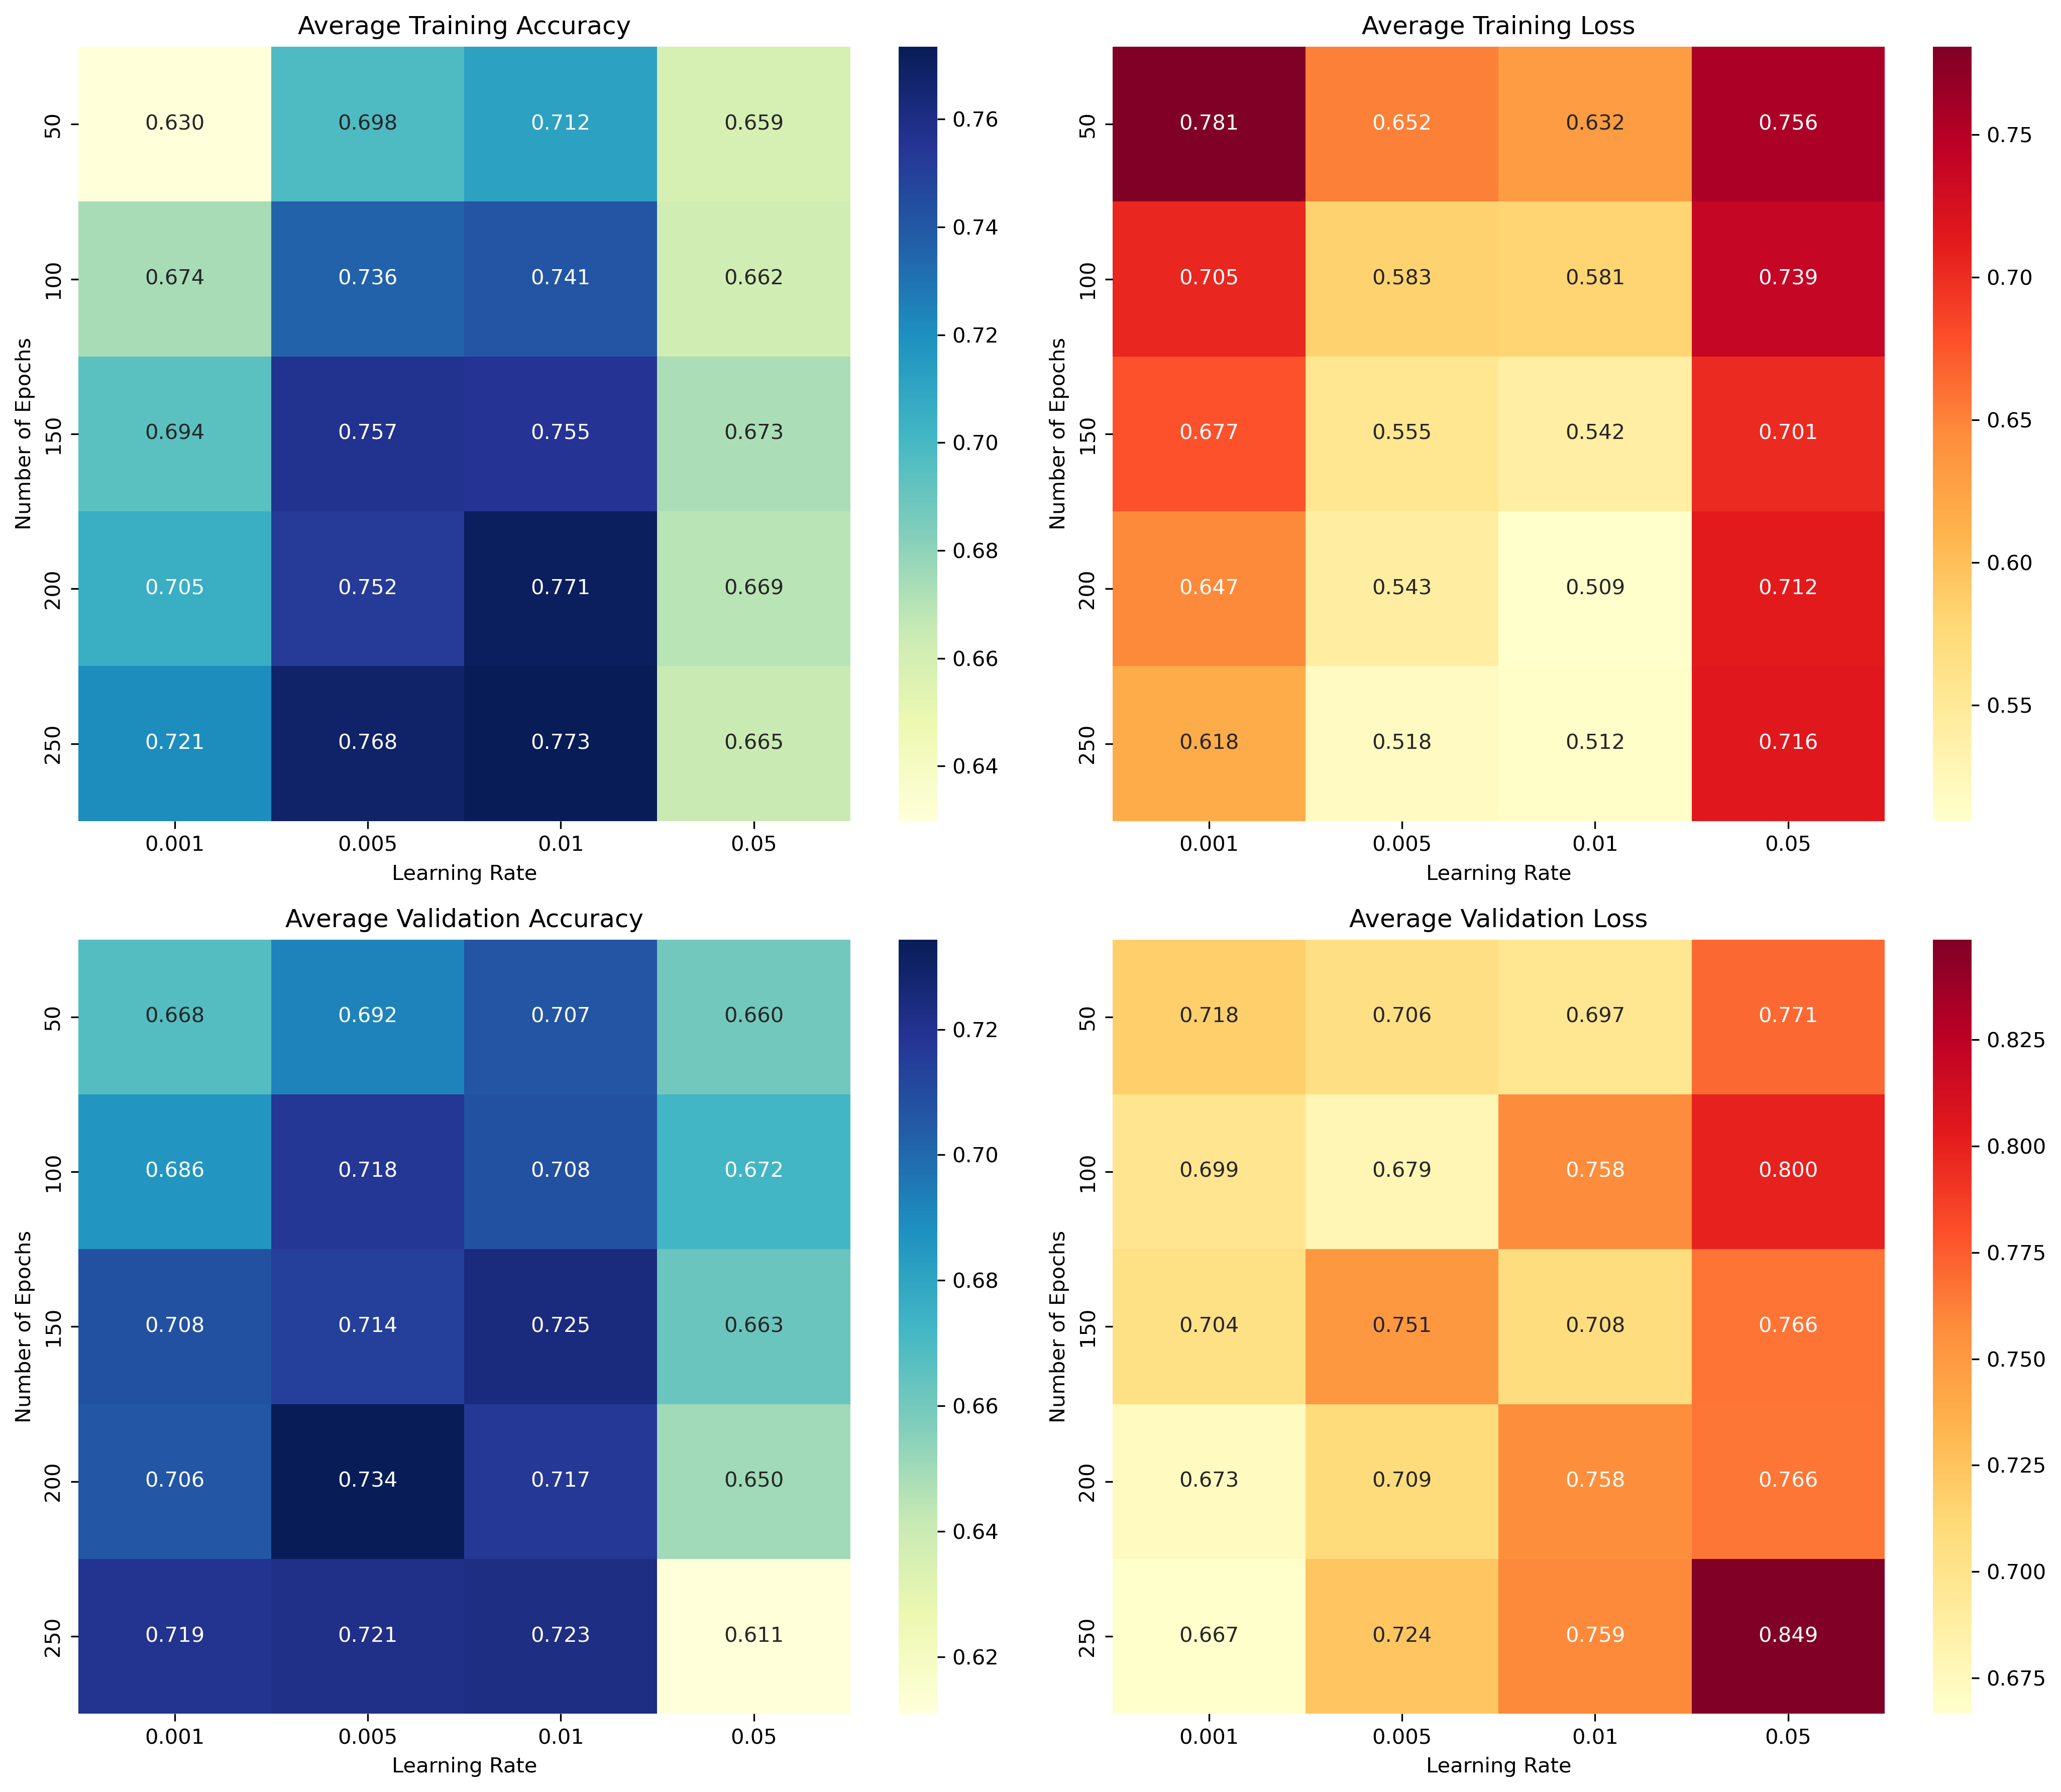
\includegraphics[width=0.8\textwidth]{./images/GridSearch_ADAM.png}  % Adjust the width as needed
    \caption{Adam Grid Search}  % Caption for the image
    \label{fig:sample_image}  % Label for referencing the figure
\end{figure*}
\subsection{Discussion and Conclusion}
It is quite clear that the results were not too great across the board, particularly in terms of loss and accuracy. That said it is clear that Adam out performed the other training algorithms rather clearly. I could argue that this may be due to something that I did wrong however this does fall in line with the fact that Adam is one of the more modern adaptive approaches, and while I would like to make a definitive statement with regards to which algorithms better. I simply can not with these results. Perhaps looking at optimizing soem other parameters such as NN architecture or momentum would provide better results. However oddly enough I dont think this was a failuire in its entirety. For some reason the hybrid appears to have performed on par in turns of accuracy with Adam. Perhaps Adam has a greater affect than I initially thought.

Hyperparameter optimization did however demonstrate a clear improvement in the results. This can be seen in the heatmaps for Adam. It is quite clear that I undershot the number of epochs in the base case and perhaps this is the case for some of the other values. This clearly indicates the usefulness of hyper parameter optimization and I suspect that if I had included a greater range in the grid search we could have seen 80\% accuracy.

In conclusion, while the overall results were mixed, there were positive takeaways, particularly from Adam, hybrid learning and the benefits of hyperparameter optimization. Future work should focus on deeper exploration of parameter tuning and network architectures to further enhance performance.

\bibliographystyle{plain}  % Choose a bibliography style (plain, alpha, abbrv, etc.)
\bibliography{references}

\end{document}
